\documentclass[a4paper]{paper} 
%\usepackage{babel}
\usepackage{hyperref}
\usepackage{amsfonts}
\usepackage{amsmath}
\usepackage{graphicx}
\usepackage[space]{grffile}
\usepackage[margin=2.5cm]{geometry}
\usepackage{pdfpages}
%\usepackage{graphicx}
\usepackage[capitalize,noabbrev]{cleveref}

\DeclareMathOperator*{\argmax}{arg\,max}

\graphicspath{{img/}}
\title{Improve path finding in the Lightning Network with the Health Improvement Algorithm}
\subtitle{Draft version}
\author{Rene Pickhardt} 
\institution{NTNU Gjovik} 

\begin{document} 
\twocolumn[\maketitle 
\hrule 
\begin{abstract}
  We introduce a health measure for the lightning network that is created from the overall health of single participants.
  The health of a node is defined of how even the funds of the node are distributed over its channels.
  We provide a re-balancing algorithm together with a communications protocol that allows a subset of nodes to improve their health.
  We test if all participants should be interested in joining to follow this health improvement algorithm.
  We measure started from unhealthy and unbalanced networks how quickly the network improves its health.
\end{abstract}

\begin{keywords}
Optimization, convex optimization, Bitcoin, Lightning Network, payment channel networks, path finding, routing, liquidity, flow control, congestion control, game theory, uncertainty, simulations, agent based systems, collaborative problem solving, 
\end{keywords}
\hrule\bigskip
]

\section{Introduction}
A major problem within privacy aware payment channel networks such as the lightning network is that the local balance of channels is not being shared with the rest of the network.
For privacy reasons the transport layer for routing payments is a source based onion routing scheme like the Sphinx Mix format \cite{danezis2009sphinx}.
Thus finding a path through the network is currently achieved by probing paths until one is found in which each channel has enough local liquidity to forward the payment.
It has been shown that probing for paths can take up to several minutes including 100 or more tries.\cite{decker2019lnconf}

One suggestion is that nodes on the lightning network could proactively re-balance their channels.
If the channel capacity was always perfectly split in half as the local balance path finding would in fact become as trivial as computing Dijkstra's algorithm.
It is trivial to see that neither initially nor after conducting payments the funds are distributed evenly among the participants so that we cannot have the goal to design an algorithm that helps to re-balance the funds fully evenly without asking participants to give money to other participants for fee which obviously is economically infeasible. 

We introduce a local and a global health measure for privacy aware payment channel networks which nodes can work towards achieving.
\section{Related Work}
While the Lightning Network White paper \cite{poon2016bitcoin} does not discuss path finding and states routing as an easy problem it is generally recognized that pathfinding on the lightning network is a difficult problem \cite{piatkivskyi2018split}, \cite{prihodko2016flare}, \cite{bagaria2019boomerang}, \cite{pickhardt2019pathfinding}, \cite{grunspan2018ant}, \cite{sivaraman2018routing}.
There is already research being conducted in the field of rebalancing channels \cite{khalil2017revive} which was more about the cryptographic protocols used to make sure that participants can enforcethe rebalancing that was agreed upon.
There are rebalancing operations for c-lightning\footnote{\url{https://github.com/lightningd/plugins/tree/master/rebalance}} and for lnd\footnote{\url{https://github.com/bitromortac/lndmanage}}.
In particular the idea of Just in time rebalancing while fulfilling routing requsts \cite{pickhardt2019jit} is already being implemented for c-lightning\footnote{\url{https://github.com/lightningd/plugins/pull/66}}. 

\textbf{TODO:} Add statistical papers of the lightning network. Payment reliability and path finding methods (similar to PhD Proposal)


\section{Formalization and Assumptions}

Let $G=(N,E,c)$ be a privacy aware payment channel network with a finit set of nodes.
The payment channels are the edges in the network such that $E\subset N\times N$.
Additionally we have a publicly known capacity function $c: E\longrightarrow \mathbb{N}$ that assigns a capacity to every edge of the network.
For every edge $e=(u,v)$ we denote $e_u:=(e,u)$ as the first participant of the channel and $e_v=(e,v)$ as the second participant.
Every node can be assigned its set of channels which we encode with the neighbor function $n : N \longrightarrow 2^{E}$.
Similarly, if we want to denote the set of neighboring nodes we use the function $n_n : N \longrightarrow 2^{N}$.
Naturally, the capacity of every channel $e=(u,v)$ is privately split into the local balances with the balance function $b: E\times N\longrightarrow\mathbb{N}$ such that $b(e_u)+b(e_v)\stackrel{!}{=}c(e)$.

We define the channel balance coefficient for $u$ on the channel $e=(u,v)$ as  $\zeta_{(u,v)} = \frac{b(e_u)}{c(e)}$.
This is just the relative amount of funds that participant $u$ has in the channel $e$.
Note since $b(e_u)+b(e_v)\stackrel{!}{=}c(e)$ we also have $\zeta_{(u,v)} + \zeta_{(v,u)}=1$

To make the following formulas easier to read we set $U:=n_n(u)$ the set of channel partners of participant $u$.
The total funds of a participant $u$ are denoted as $\tau_u:=\displaystyle{\sum_{e\in U}b(e_u)}$.
The values of $\tau_u$ will be constant while the balance function $b$ is pertubed.
Similarly the total capacity of a participant $u$ is denoted as $\kappa_u:=\displaystyle{\sum_{e\in U}c(u)}$.
Using the last two definitions we can define the node balance coefficient for a participant $u$ as $\nu_u = \frac{\tau_u}{\kappa_u}$.

We define a node $u$ healthy if its channel balance coefficients $\zeta_{(u,v_1),\dots,\zeta_{(u,v_d)}}$ have the same value.
This means that the relative distribution of a nodes funds across all its channels is the same.
Consequently, we consider a node unhealthy if it local channel balance coefficients are unequal.
Statistically inequality of a distribution is meassured with the Gini coefficient.
Thus for a node $u$ with channel balance coefficients $\zeta_{(u,v_1),\dots,\zeta_{(u,v_d)}}$ we define $G_u = \frac{\displaystyle{\sum_{i\in U} \sum_{j \in U}} | \zeta_i - \zeta_j |}{2 \displaystyle{\sum_{i \in U} \sum_{j \in U} \zeta_j}}$
If $G_u = 0$ this means that the channel balance coefficents are equal which we considered as health.
In contrast if $G_u = 1$ the channel balance coefficients are distributed in the most unequal way meaning the node is unhealthy.

It is worthwhile to mention and easy to see that the Ginicoefficient of the channel balance coefficients of a node $u$ takes the value $0$ if and only if its channel balance coefficents all take the same value.
This value will be exactly the same as the node's balance coefficient $\zeta_u$. \footnote{formaly proove this? This will be used in the rebalance algorithm to compute the rebalance amount. so maybe move? }

Finally the health of the network as $H = \displaystyle{\frac{1}{|N|}\sum_{n\in N}G_n}$ which is just the mean of the health values of all nodes in the network.
Again a perfect health of the network would be achieved if $H$ takes the value of $0$ where as the health is poor if the value of $H$ is close to 1.

Our goal is to find a balance function $b$ which minimizes $H$ given a parivacy aware payment channel network with initial distribution of funds $\tau_{u_1},\dots,\tau_{u_n}$.
The constraint to this optimization problem that the total funds $\tau_u$ are fixed for every node $u \in N$ and any choice of the balance function $b$.
As we are in a privacy aware payment channel network the distribution of funds $\tau_{u_1}\dots,\tau_{u_n}$ is not publically known.\footnote{While the initial distribution could be guessed from the funding transactions in the case of the Bitcoin Lightning Network for public channels this distribution will also change with the first payment that is not a rebalancing operation.}
In the same way the initial balance function is not publically known.
As we lacking knowledge we cannot aply standard optimization techniques like gradient descent, conjugate gradient methods or simulated annealing.
We suggest to use an agent based heuristic in which every participant executes some operations to improve its own help which others support if it also improves their health.
Before we describe our proposed algorithm in \ref{sec:Algorithm} we will now see a small example of our terminology. 

\subsection{Example}
\begin{figure}
 \centering
 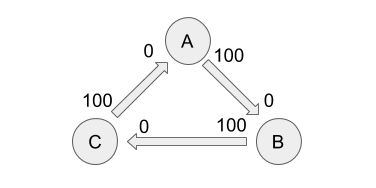
\includegraphics[width=8cm]{img/evenUnbalanced.png}
 \caption{A, B and C all own 100 satoshi.}
 \label{fig:evenUnbalanced}
\end{figure}
In Figure \ref{fig:evenUnbalanced} you can see an a small network consisting of $3$ nodes in which the balance are distributed unevenly.
The global balance coefficients for every node are $\nu_u=0.5$.
The $\zeta$ values for each node are $0$ for the channel in which the node owns no funds and $1$ for the channel in which the node owns all the funds.
This leads to a local health for every node of $0.5$ and a global health of the network of $0.5$.
\begin{figure}
 \centering
 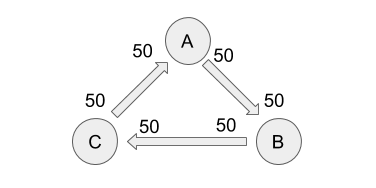
\includegraphics[width=8cm]{img/evenBalanced.png}
 \caption{Each node still owns 100 satoshi but distributed evenly balanced amonth their channels}
 \label{fig:evenBalanced}
\end{figure}
Now in Figure \ref{fig:evenBalanced} we see the balanced view of this network.
The total funds $\tau_u$ stayed constant as it is the constrain of the optimization problem.
However since the funds have been rebalanced the local balance coefficients $\zeta$ of every channel now take the value of $0.5$ leading to a local health coefficient $G_u=0$ for every node $u\in N$.
This in turn leads to a perfectly health network with $H=0$.

Considering multi path payments in both cases of the network every node was able to pay the full funds they owned to every other participant.
If the edge $e=(A,B)$ was removed in the halthy network $A$ would still be able to pay $B$ with a path over $C$.
This would not be possible in the unhealthy network as the funds where distributed poorly.
It is worthwhile to mention that not every network can achieve a perfect global health $H=0$.
\begin{figure}
 \centering
 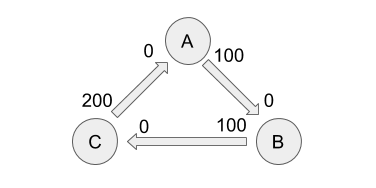
\includegraphics[width=8cm]{img/oddUnbalanced.png}
 \caption{Example of an unbalanced network that does not allow for perfect balance as funds are not distributed evenly.}
 \label{fig:oddUnbalanced}
\end{figure}
For example let us look at figure \ref{fig:oddUnbalanced} we see due to the fact that the total funds are not distributed evenly (node $D$ owns twice as many funds as the others.

\begin{figure}
 \centering
 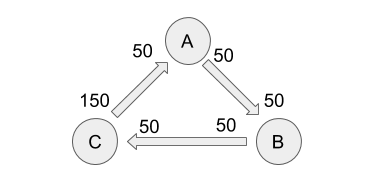
\includegraphics[width=8cm]{img/oddBalanced.png}
 \caption{Best possible balance in a network for which the funds are not distributed equally.}
 \label{fig:oddBalanced}
\end{figure}
That there can also be no perfect rebalancing of funds resulting in figure \ref{fig:oddBalanced}.

\subsection{Description of the algorithm}\label{sec:Algorithm}
As stated before we suggest an agent based heuristic in which participants can use the local knowledge they have in order approach the global optimization problem of finding $b$ such that the health of the network is good.

\begin{enumerate}
\item A node $u$ will compute its node balance coefficient $\nu_u$.
\item $u$ will then compute the channel balance coefficients $\zeta_{(u,v_1)},\dots,\zeta_{(u,v_d)}$ for its $d$ channels.
\item The node will select all channels $e=(u,v_i)$ for which its channel balance coefficient is higher than its node balance coeffient i.e $C = \{(u,v_i) | \zeta_{(u,v_i)} - \nu_u\ > 0\}$.\footnote{Note that we do not need to take absolute values as $u$ will only be able to initiate a rebalancing operation by sending money which means decreasing its cannel balance coefficient of $\zeta_{(u,v_i)}$}.
\item from the candidate set $C$ a random channel $e=(u,v)$ is selected.\footnote{We show in the experimental evaluation that always taking the channel with the biggest gain makes the heuristic stuck too quickly. The reason is that if a channel cannot be rebalanced in the next step the same channel is tried again.} 
\item Now the node searches for a circular payment to itself along $e=(u,v)$ by choosing a path $p = [u,v,x_1,\dots,x_n,u$. The amount of that payment should decrese the value of $\zeta_{(u,v)}$ to that of $\nu_u$ and can be computed as $a = c(e)\cdot (\zeta_{(u,v)}-\nu_u)$. Also the end of the circle should be a channel $(u,x_n)$ for which the channel balance coefficient $\zeta_{(u,x_n)}$ is smaller than the node balance coefficient $\nu_u$.
\item the node will conduct the payment if the nodes on the path $p$ agree to do this payment. 
 \item Repeat all steps as long as the local balance coefficients are still not even.
\end{enumerate}

In case a circular path exist it is easy to see that the making a payment along this path will make the distribution of local balance coefficients for node $u$ more even.
If no such circle can be found the local health is staying constant.
Obviously finding a circular rebalancing path is tricky as the balances of the network are not known and this will again boil down to probing as it is done currently in the lightning network for regular payments..
Also rebalancing might worsen the health of another node along the path in in that way not actually contributing to improve the global health.
The biggest drawback is that in the current implementation of the Lightning Network such a circular payment will cost the initator some routing fee which economically deincentivizes the node to improve its health even though our evaluation suggest that it will be benefitial for the network.

\subsubsection{Adoptions to the communication protocol}
In order to get rid of these problems we suggest to extend the communication protocol between channel partners and to update the algorithm.
.We take the idea of cost free rebalancing in the friend of a friend network as it was first proposed in the context of JIT-Routing \cite{pickhardt2019jit}.
In order to calculate a circular path node $u$ will query $v$ for the channels on which $v$ would be willing to forward the amount $a$ in a circular way.
$v$ will only return channels potentially with a lower amount than $x$ on which it  would also improove its local health $G_{v}$.
In the same way $u$ will ask the nodes though which channels it would like to receive the funds on which channels they would like to receive funds in a circular way to improve their health.
Both querries will allow the nodes to signal that they will be willing to participate in a rebalancing operation for up to $x$ tokens.
After the node $u$ has aquired this subset of channels in its friend of a friend network it searches for a path from $v$ to $u$.
This path will be preceeded with the first hop from $u$ to $v$ making it a circular payment.
The amount send on this circular payment will be the highest possible value up to $x$
Nodes will drop the routing fees for this circular path as it will improve the health of each node and provie a direct benefite instead of a routing service.

From a privacy point of view revealing channels on which a node is willing to participate in a rebalance operation to its neighbors does not directly leak more information than could be probed anyway.
Also nodes don't have to answer to the queries truethfully and could always intrudize some fuzziness for privacy reasons. 
While we suggest that channel partners share some information with each other this is not necessary for the algorithm to work.
First of all nodes can probe for rebalancing circles that are benifitial for itself.
Second s nodes on the way would only fulfill the fee free rebalncing request if it also improves their health this algorithm could work without actively sharing information in the friend of a friend network.

\section{Experimental Setup}
We generate synthetic graphs of various sizes and always initialize them with the full capacity on one side of the channel.
We then conduct a simulation of the algorithm in the following way:
\begin{enumerate}
\item Assign $C$ as the candidate set of all nodes in the network.
\item As long as $|C| > 0$ do the following steps.
\item A random node from $C$ is chosen and is allowed to do one rebalancing operation to improve its network health.
\item If the node was successfull go back to step $1$.
\item If the node could not improve its health remove the node from $C$ and go to step $3$.
\end{enumerate}

This setup is slightly modified to answer several questions:

\subsection{Well definition of the globl health measure}
The initial setup is conducted for various networks of various sizes with the goal of measuring how the overall health of the network improves.
We will test if the the Ginicoefficients of the nodes are distributed normally such that measuring the global health of the network as the average does actually make sense.
These experiments are also made to see how much work it takes nodes to execute their rebalancing operations and improoving their local health.
We shall also see if the algorithm always converges.

\subsection{Onboarding phase}
If this method becomes part of the lightning network implemntations not all nodes will update their software at the same time.
Thus we conduct the simulation again on the same networks but only with a fraction of nodes engaging in the health improvement algorithm.
We wish to examine how the overall health of the network depends on the participation of nodes.
For this we will actually do a second experiment in which the rebalancing can still take place over nodes that did not participate in the algorithm.
This can be achieved by paying regular routing fees.

\subsection{Real time changes of funds allocation}
As making a regular payment, opening or closing a channel changes the funds distribution of the network $\tau_{u_1},\dots,\tau_{u_n}$ the health improvement algorithm will be pertubed and have a different optimal solution.
We want to see how such operations impact the health improvement algorithm and how quickly the algorithm can adjust to such changes to the allocation of funds.
Thus with a likelihood of varying $p$ we mix Lightning Network operations like making payments as well as adding and removing channels to the simulation.
We will test the ratio of rebalancing operations to payments on the network for the network to stay healthy and be able to fullfill payments.
This will give us a hint how much overhead will come from the health improvement algorithm in order to be useful and if it is feasible to execute the algorithm.


% ==========================================================
\section{Results}

\begin{figure}
 \centering
 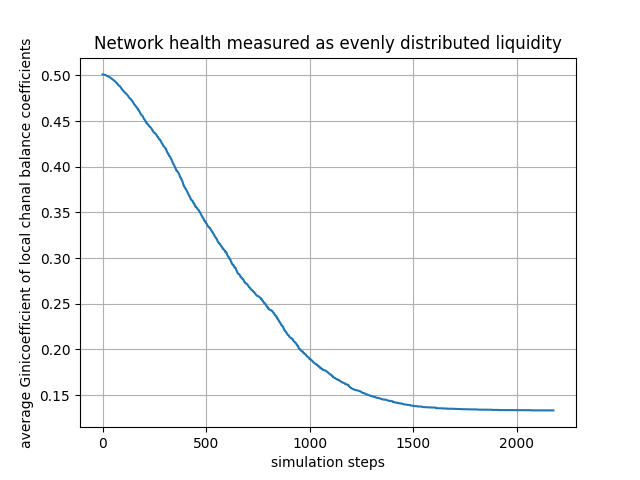
\includegraphics[width=7cm]{code/results/routabilityTest/1574847007_figure.png}
 \caption{Health evolving with execution of the algorithm on a network with 101 nodes and 1788 edges. The edges have been initialised with uniformly distributed capacities between $1000$ and $10000$ satoshi. Ihe full capacity is initially with the funder of the channel.}
 \label{fig:healthovertime}
\end{figure}

\cref{fig:healthovertime} confirms that the health score of the network is decreasing over time when running our simulation.
This means that the network is becoming more balanced or healthier.
We see that most improvement is happening quite fast with a few simulation steps.
On average, each node had attempted to rebalance at least $n$ times, where $n$ is the count of the node's payment channels.
This seams plausible in the sense that every channel gets rebalanced at least once.\footnote{Note that due to the collaborative behaviour of nodes a node also gets channel rebalanced in the rebalancing attempts of other nodes.} 
In particular the algorithm converges in a local minimum rather quickly.
Note, that the established minimum is a local minimum. 
Our experimental runs resulted in states that are not identical, however, the differences were negligible. 
We can therefore assume that the local minimum might be close to global minimum as the collected data demonstrate.

\begin{figure}
 \centering
 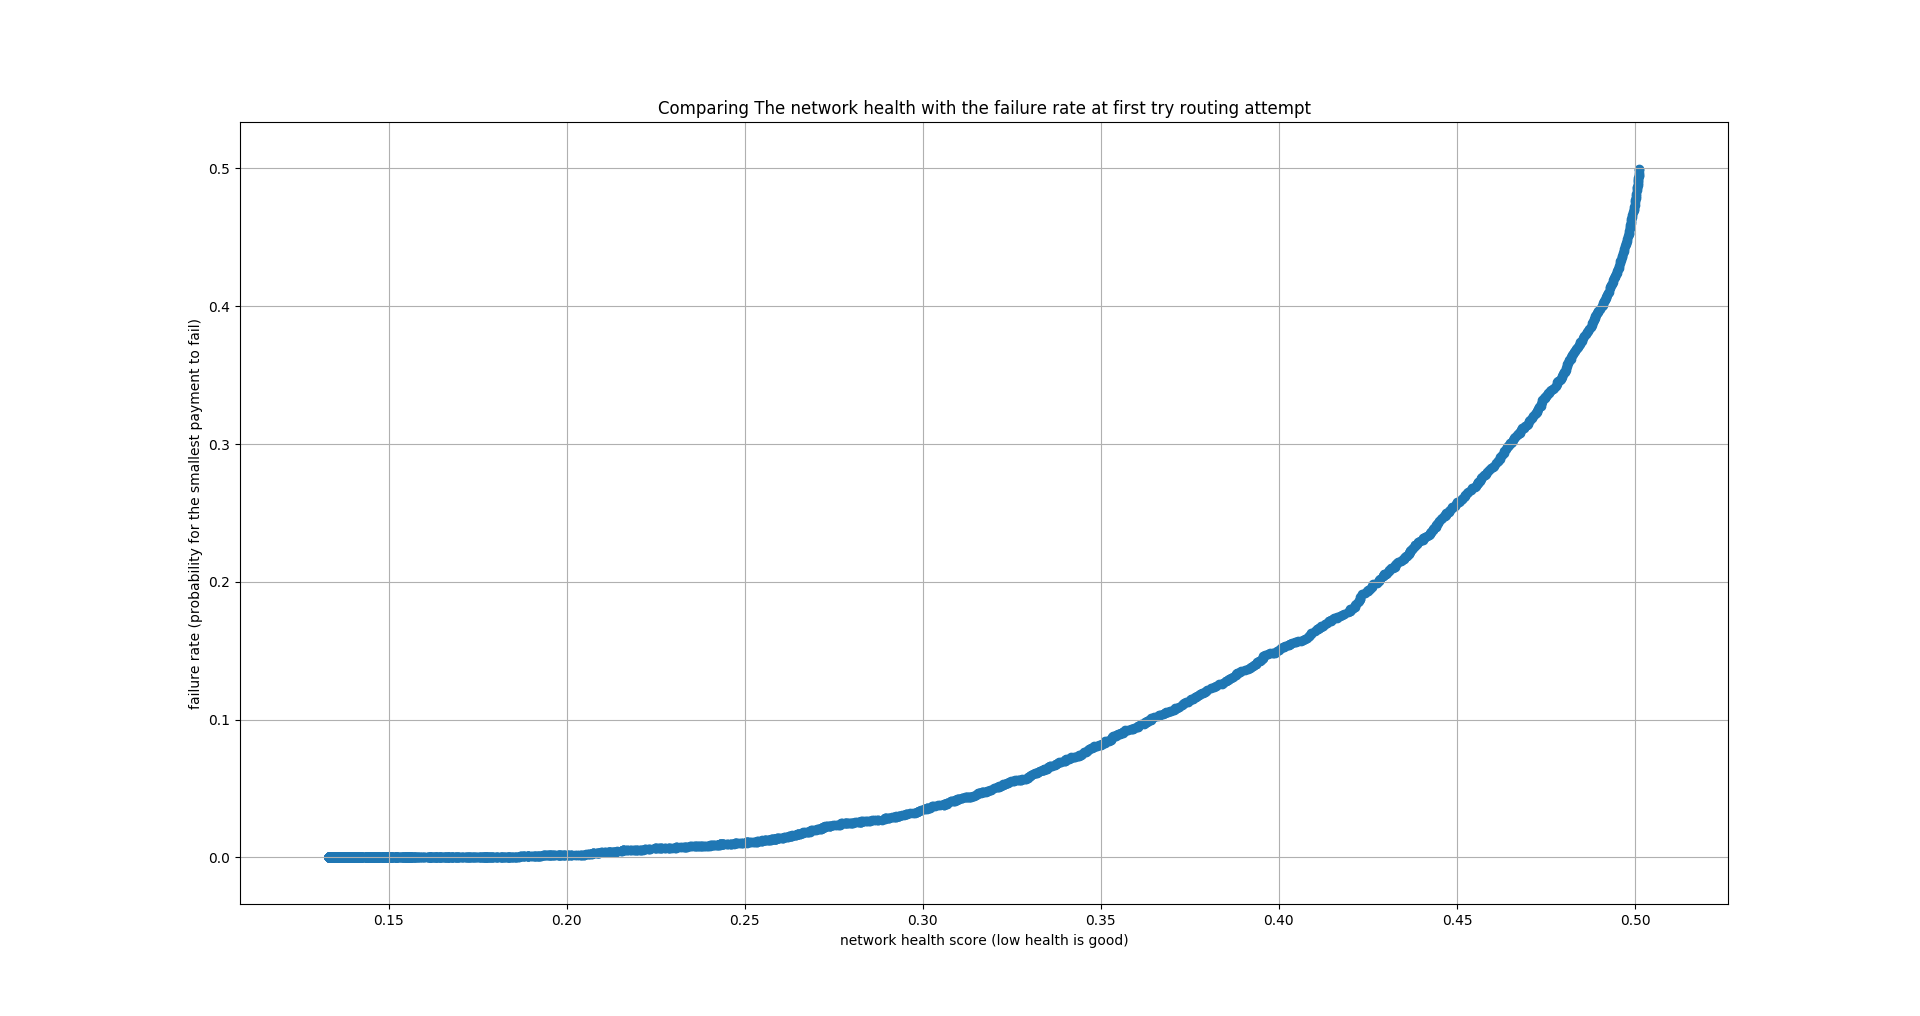
\includegraphics[width=8cm]{code/results/routabilityTest/health vs payment rate.png}
 \caption{For every step of the simulation the health of the network is plotted against the probability for a random payment of the smallest possible amount to fail.}
 \label{fig:healthVsFailurerate}
\end{figure}

In \cref{fig:healthVsFailurerate} we compare our defined health score with the failure rate of payments.
We can see that better (lower) health scores yield a lower failure rate for payments.
The failure rate is measured by attempting a payment between all pairs of nodes and counting the relative amount of payments that cannot be routed on the first selected path from the payment channel network.
We calculate the failure rate and the health score after every simulation step and plot the points as a scatter plot.
This result confirms the dependency of the payment failure and the worse health indicator. It is the first experiment that indicates that the defined health score is semantically correct and well chosen. 

The goal of the second experiment is to check if the overall amounts that can be routed increase with better (lower) health scores.

\begin{figure}
 \centering
 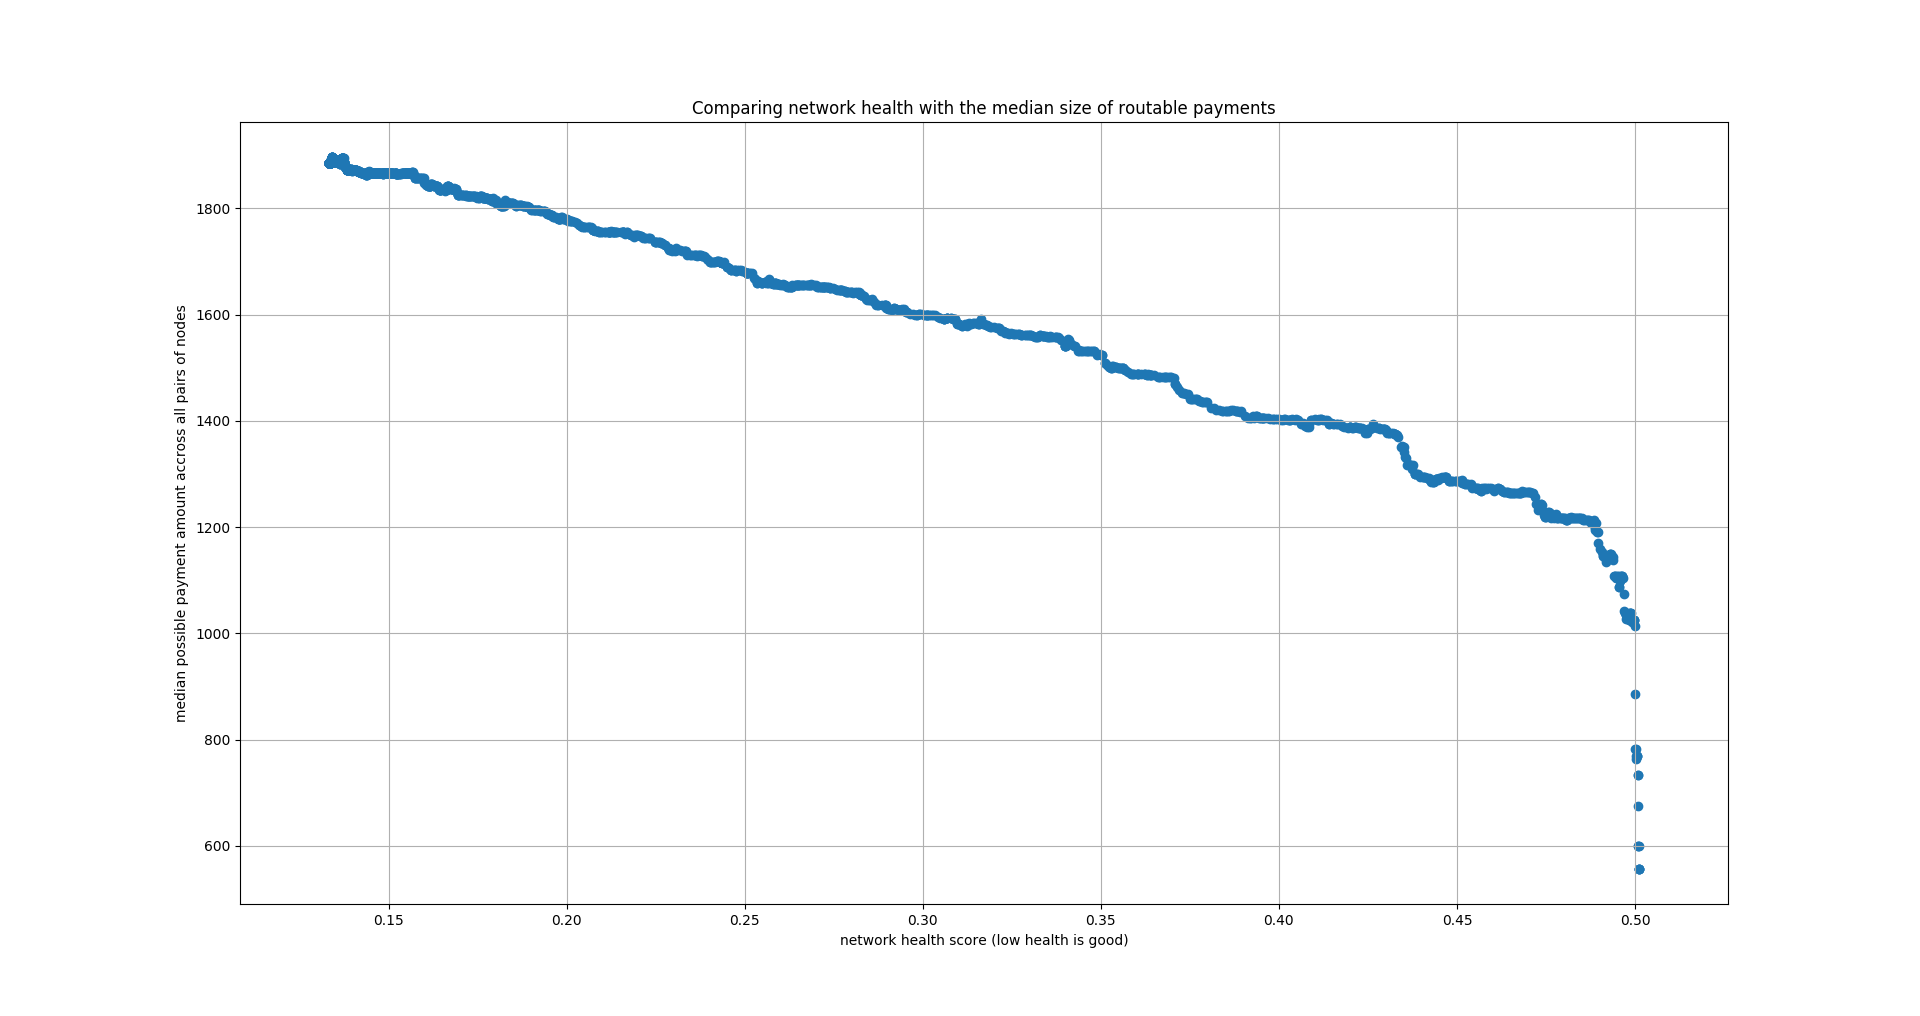
\includegraphics[width=8cm]{code/results/routabilityTest/health vs payment amt.png}
 \caption{For every step of the simulation the health of the network is plotted against the median value of payments that can be fulfilled. Note that failed payments are part of the statistics and counted as payments which can send $0$ satoshi.}
 \label{fig:healthVsPayment}
\end{figure}

In \cref{fig:healthVsPayment} we compare the health score with the median payment amount.
The median payment amount is computed as follows.
First all pair of shortest paths are computed.
We then look at the amount that could actually be forwarded through each path.
Finally we take the median of those amounts.
This means that at least $50\%$ of payment pairs are able to forward this amount.
The higher this amount is the higher payments are supported by the network.
We see a nice negative correlation between the health score and the median routable payment amount.
This suggests that a healthier network is statistically able to route higher payment amounts on the first try.
This is particularly important as privacy aware payment channel networks use source based onion routing and technically have to guess a path. When those initially guessed paths provide a low failure rate with high payment amounts there are considerable benefits for the overall functioning of the payment network. 
The user experience is improved, the payment delays are lowered, and the amount of messaging and coordination is minimised. 

\begin{figure}
 \centering
 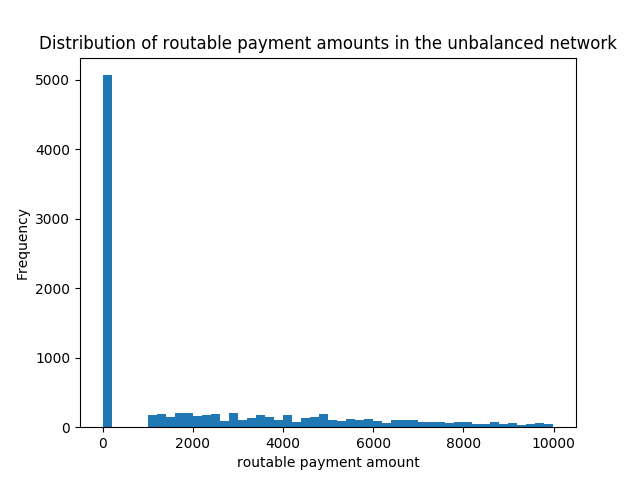
\includegraphics[width=8cm]{code/results/routabilityTest/paymentamtUnbalanced.png}
 \caption{The initial distribution of maximum payment amounts that are possible to be paid on the first routing attempt between all pairs of nodes in the network.}
 \label{fig:paymentUnbalanced}
\end{figure}

\begin{figure}
 \centering
 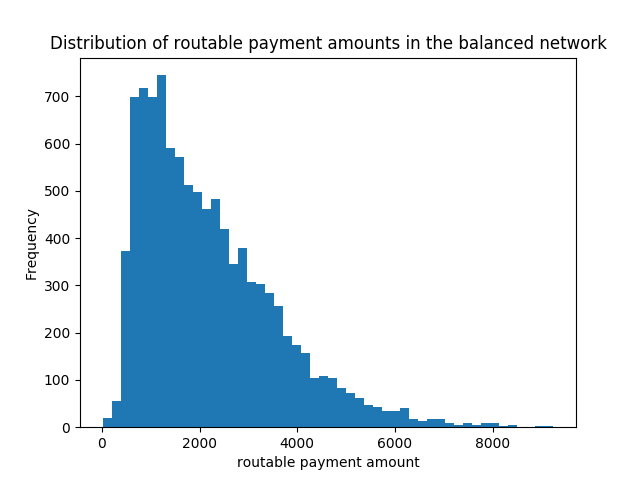
\includegraphics[width=8cm]{code/results/routabilityTest/paymentamtBalanced.png}
 \caption{The final distribution of maximum payment amounts that are possible to be paid on the first routing attempt between all pairs of nodes in the network after the health improving algorithm has converged into a local minimum.}
 \label{fig:paymentBalanced}
\end{figure}

To demonstrate that the median actually makes sense we depict the distribution of possible payment amounts between all pairs of nodes on the unbalanced network which we used as an input for the algorithm in \cref{fig:paymentUnbalanced} and also the distribution of possible. payment amounts on the balanced network after the algorithm has been executed successfully in \cref{fig:paymentBalanced}.

Finally, we have tested, from a statistical point of view, a validity of computing the health as the average of the local health coefficients.
To test that, we verified if the local health coefficients $\nu_u$ for all $u \in N$ follow a normal distribution. This has been successfully confirmed with the D'Agostino normallity test~ß\cite{d1971omnibus}.
This test achieved a p-value of $0.027$ on the balanced network.
One can see in \cref{fig:giniStart} and \cref{fig:giniEnd} how the distribution of local health coefficients looks before and after rebalancing the network. We can see that, on average, the mean of the distribution is being decreased. This is to be expected. 

\begin{figure}
 \centering
 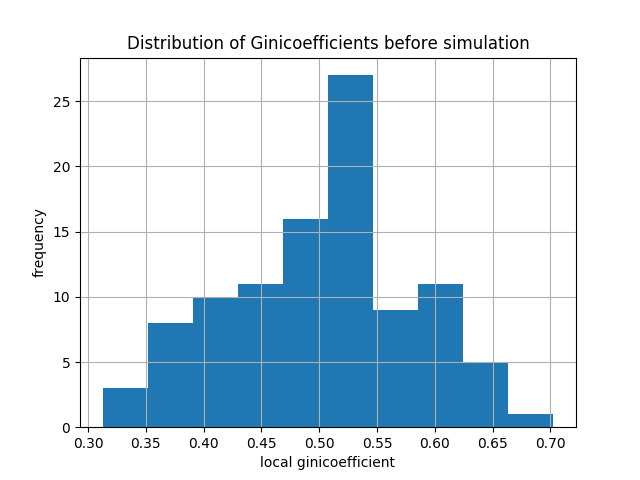
\includegraphics[width=7cm]{code/results/routabilityTest/1574847007_ginicoefficients_start.png}
 \caption{The distribution of Gini-coefficients (local health coefficients) in the unbalanced random network before the simulation started.}
 \label{fig:giniStart}
\end{figure}ß
\begin{figure}
 \centering
 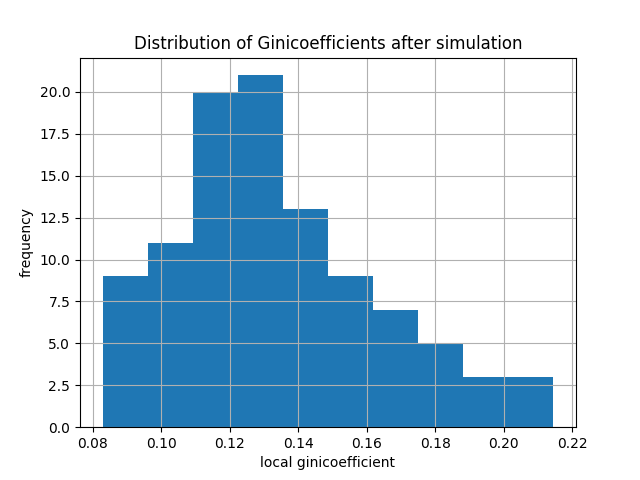
\includegraphics[width=7cm]{code/results/routabilityTest/1574847007_ginicoefficients_end.png}
 \caption{Distribution of Gini-coefficients (local health coefficients) for all nodes in the random network after the health improvement algorithm successfully executed.}
 \label{fig:giniEnd}
\end{figure}


%show (compute!) histograph of the unbalanced and balanced network of payment amounts to make more sense of the median measure
% actually it would be nice to do a kolmogorov smirnof test on distributions by comparing the L_1 norm of the CDFs


% =======================================================================
\section{Future Work}

We want to study if the optimization problem is convex and thus the local minima is also a global minima.
Does our algorithm always find the local / global minima?
Find an algorithm that does produce the global minium.
Concurrent payments / rebalancing operations within the simulation

difference between I pay for a circular onion to get my node in perfect health vs. we do a fee free rebalancing but I must accept that other nodes might not want to rebalance the entire amount that I am suggesting.

Multipath rebalancing! if thirty needs to send out maybe one channel needs 10 in and the other one 20. If it is not multipath it will need two rebalncing operations. Especially when having FOAF talking one could already split this and make several requests.

Having different strategies to define local health. How does the algorithm generalize? 

Note while we empirically verified that the health measure increases the overall ability of network participants to route payments on random paths the health measure has some edge cases in which it is breaking with the intuitive semantics a person would have.
Consider for example a node that opens $d$ channels and has all the funds on its side.
In that case the local channel coefficients $\zeta_{(u,v_1)},\dots,\zeta_{(u,v_d)}$ would all take the value of $1$ resulting in $G_0 = 0$ meaning this node is in perfect health.
However from a network perspective this node could node forward any payments and cannot even be rebalanced unless the overall topology changes by either $u$ making a payment or another node opening a channel with $u$.
Thus a future work in the direction of autopilots and channel management might include to not only optimize ones node for a low value of $G_u$ but also to optimize towards $\nu_u = 0.5$.

In section we have mentioned that besides the communication protocol to share informations about channels there needs to be a transport mechanism for fee free circular payments.
Obviously the onions could not be reused as a node might steal routing fees and hide them as a rebalancing request.
This paper did not discuss the crypotgraphic protocols necessary to ensure that a proovably fee free rebalancing operation can be executed.
While approaches for blockchains with more expressive scripting languages exist \cite{khalil2017revive} we leave it as a future work to provide a cryptographic protocol to be able to fulfill these requests in bitcoin.

\section{Conclusion and Discussion}

Also nodes might want to define their health in a different way thatn comparing the local balance coefficients to their global balance coefficients.
For example routing nodes or liquidity providers might very well want to have high values of $\zeta$ on some of their channels where as they might be willing to accept low values for $\zeta$ on other channels.
In a similar way merchants will probably prefer many channels with low values of $\zeta$.
The algorithm could very well be exchanged to a version in which nodes decide their own health metric.


The overall flow, liquidity and ability to route payments successfully on the first attempt is higher in well balanced networks. 
The results suggest that nodes have an interest to increase their own health and to take part in rebalancing operations of other nodes if that benefits the own health of the node.
As balances of channels in the frien of a friend network can easily be probed it seems plausible in privacy aware payment channel networks to include a communication protocol with which a node signal their partners that it wants to rebalance a certain channel with a certain amount and ask them which of their channels are interesting for supporting such a rebalance operation.
We suggest that payment channel networks introduce a mechanism of fee free rebalancing if the rebalancing operation if every hop along the circle believes that the rebalancing operation is benefitial to them. 


\bibliography{lightningNetworkHealth}
\bibliographystyle{plain}

\end {document}
